\documentclass{article}
\usepackage{amsmath, amssymb, mathtools, runcode, verbatim, tikz, graphicx}
\usepackage[margin=1in]{geometry}
\title{Automatic SAS hierarchical analysis instructions}
\begin{document}
\maketitle
\section{Structure}
There are two main components, a classifier and a regressor.
The classifer is a hierarchical structure, and has some weird quirks, stemming from 5 distinct support vector classifiers each with their own hyperparameters.
The are in fact several different regressors, each of which have their own hyperparameters.
These should work fine, as they are.
The classifier is defined in the file \texttt{hierarchical.py} in the \texttt{hierarchical} directory.
The regressors are defined in the \texttt{sas\_krr\_reg.py} file in the \texttt{krr} directory.
They are both invoked and called in the \texttt{full\_send.py} file in the \texttt{full\_medul} directory.
This file contains a decent example of using both of them, but there is a bunch of other stuff too, such as printing output files.
One last really important file is \texttt{loaders.py} This contains functions for loading all data, which will be important.

\section{Classifier}
The classifier is a little weird. Currently the constructor for an instance of a classification tree takes the structure as an argument to allow for experimenting with the optimal architecture. That isn't something that we should be dealing with in the visualition aspect. I would reccomend just copying and pasting the description from \texttt{full\_send.py}.
%\showCode{python}{full\_model/full\_send.py}[118][124]
\begin{verbatim}
    decision1 = {0:0,1:0,2:1,3:0,4:0,5:1}
    decision2 = {0:0,1:0,3:1,4:1}
    decision3 = {0:0,1:1}
    decision4 = {3:0,4:1}
    decision5 = {2:0,5:1}
    decisions = [decision1, decision2, decision3, decision4, decision5]
    hierarchical_map = [{0:1,1:4},{0:2,1:3},{0:'0',1:'1'},{0:'3',1:'4'},{0:'2',1:'5'}]
\end{verbatim}
The dictionary maps a true class to the output class of that decision. 
The first one is the first decision separating cylinders (0), disk (1), core shell cylinders (3), and core shell disks (4), from spheres (2) and core shell spheres (5).
The second decision separates cylinders, and disks from cs cylinders nd cs disks.
The third decision separates cylinders from disks.
The fourth decision separates cs cylinders from cs disks.
The fifth decision separates spheres from cs spheres.
A summary is shown if figure \ref{fig:tree}

\begin{figure}
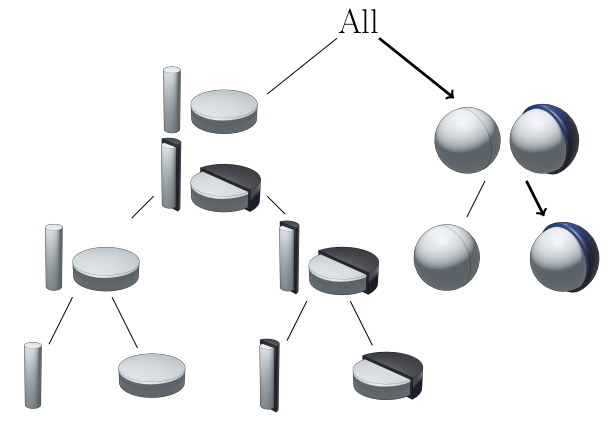
\includegraphics[width=\linewidth]{figs/abs-tree.png}
\caption{A diagram of the tree structure of the classifier}
\label{fig:tree}
\end{figure}

The tree is actually intantiated in the following two lines.

\begin{verbatim}
    classifiers = hier.create_classifiers(args.struct_strings, gamma_norm)
    hierarchical = hier.create_hierarchical(classifiers, decisions, spec, labels)
\end{verbatim}
The first line actually creates the SVC object from sklearn.
The secnd line organizes them using the structure defined above.
Further it traines these classifiers.  I have run into some weirdness attempting to save and reload trained svcs, but these only take a few seconds to train. 
I would reccomend training it when the server is started and then just leaving the hierarchical reference hanging out.  
It is a bit of overhead that I should fix eventually, bbut as long as we're not retrining it every time the parameters change it shouldn't affect the visualization too much.

lastly is the \texttt{eval\_hierarchical}function defined in the \texttt{hierarchical.py} file, and demonstrated in \texttt{full\_send.py}
\begin{verbatim}
    preds, mapped_labs, mapped_inds = hier.eval_hierarchical(classifiers, hierarchical_map, 
tspec, tlabels)
\end{verbatim}
This takes the classifierrs and hierarchical map trained above, as well as test spectra and test labels.
It returns, predicted classes, the labels corresponding to them, and the original index of those spectra.
It is worth noting that both the mapped\_labs, and mapped\_inds variables are the result of the hierarchical structure shuffling the data as they are evaluated.
I should as a note to self just move the handling of this into the funtion and not return these at all.
In either case the visualisation, for now should be focused on one spectra at a time, and the label will be unknown, so just ignore these. The only variable of intrest will be preds.
This will contain the predicted class of a spectra.

\section{Regression}
There are many regressions, and they require many hyperparameters, but I have them handled in a much more abstracted way.
\begin{verbatim}
    gamma_norm = train_spec[args.targets[0]].shape[0]
    regressors = construct_regressor(args.reg_file, gamma_norm)
\end{verbatim}

The gamma norm is just the number of data points in any one spectra, and the regressors ar all created using this value, as well as the regi\_file, which is the plain text file \texttt{regression-hyperparameters} in the \texttt{full\_model} directory.
This returns a dictionary of dictionaries.
The outermost dictionary is of morphologies.
The next layer is of parameters.
For example to find the regressor object for the radius of cylinders one would call \texttt{regressors['cylinder']['radius']}.
Once the morphology is predicted you will probably just want to iterate through the parameters.
\begin{verbatim}
        for p in regressors[t].keys():
            predicted_parameters[p] = regressors[t][p].predict(spec)
\end{verbatim}

\section{Loading}
The file \texttt{loaders.py} contains the functions to load files.
\begin{enumerate}
\item \texttt{load\_q}(\texttt{datadir}, \texttt{q\_file}='q\_200.txt')
Simple takes the path to the source directory where the data are saved. This is not the full filename. There is a second argument if a different file is saving the actual $q$ data, but the default should work for now.
\item \texttt{load\_params}(\texttt{filename}, \texttt{colnames})
\begin{itemize}
\item \texttt{filename} is the name of a the file in question. This should be a full or relative path.
\item \texttt{colnames} is a list of column names to load such as ['radius', 'length']
\end{itemize}
returns a dictionary mapping each column name to an array.  If the column is not present in the data an array of zeros are returned instead.
This allows the asme set of columns to be passed to all morphologies as the lack of shell or length are error handled elsewhere.
\item \texttt{load\_all\_spec}(\texttt{targets}, \texttt{q}, \texttt{datadir}, \texttt{dataset}, \texttt{prefix}='train')
\begin{itemize}
\item \texttt{targets} a list of morphologies to load.
\item \texttt{q} is an array of string for the $q$ values. These are column headers in the pandas dataframe, so keep them as strings, not floats.
\item \texttt{datadir} is the source directory of the data, I.E., "\texttt{../data}" from the \texttt{full\_model} directory.
\item \texttt{dataset} is the subset of data to use I.E., \texttt{lowar16}.
\item \texttt{prefix} defaults to 'train', but should be changed to 'test' for the evaluation data.
\end{itemize}
returns a dictionary mapping each morphology name to an array of spectra of shape ($n$,200), where $n$ is the number of spectra and 200 because there are 200 features.

\item \texttt{uravel\_dict} (\texttt{spec\_dict}, \texttt{targets}=None)
Takes the output from \texttt{load\_all\_spec} and concatenates it into one long array. The dictionary is useful for training different regressions for each morphology. The concatenated array is required to train the classification.
It also returns an array of class labels, and a map, mapping each entry in the concatenated array to its original index in the separate class arrays.
\item \texttt{scale\_highq}(\texttt{spec}, \texttt{incoherence})
\texttt{spec} is the array of spectra, either the concatenated array, or this is called separately on each class withing the dict.
\texttt{incoherence} is a depreciated argument that is ignored
\end{enumerate}

\section{Workflow}
\subsection{On Startup}
These sections should only be called once when the server is started. Some of these functions are a bit time consuming, but once these values are initialized everything should be good.
I created a new file \texttt{startup.tex} and it contains a wrapper function called \texttt{init()} this will create all the requisite objects and handle all of the training. 
Call this function once on startup.

\subsection{when a new spectra is loaded}
I demonstrate loading a new spectra called 'ex\_spec\_1.csv'. Try loading this file into the workflow.
I added two other functions called \texttt{predict\_motphology} this will return the string of the predicted morphology, and \texttt{predict\_dimensions}, which returns a dictionary of dimensions.
These should be good interfaces between the ML and visualizations.



\end{document}
